\documentclass[journal, 12pt]{IEEEtran}

% *** CITATION PACKAGES ***
%
%\usepackage{cite}https://www.overleaf.com/project/5d8e32cf8b64620001d24060
\usepackage{capt-of}%%To get the caption
\usepackage{gensymb}
\usepackage{graphicx} %package to manage images
\graphicspath{ {./images/} }
\usepackage{wrapfig}

\usepackage{amsmath}
\usepackage{amssymb}
\usepackage{hyperref}
\usepackage{lipsum}

\usepackage[style=ieee]{biblatex}
\DeclareLanguageMapping{english}{english-apa}
\addbibresource{references.bib}
\usepackage[justification=centering]{caption}

\usepackage{setspace}

\usepackage{hhline}


\usepackage{changepage} 

\usepackage{booktabs}
\usepackage{xcolor}

\usepackage{makecell}
\usepackage{graphicx,subcaption}
\usepackage{listings}
\renewcommand\theadfont{}
\DeclareMathOperator{\EX}{\mathbb{E}}% expected value


\usepackage{multicol} 

%\raggedbottom

\renewcommand{\ttdefault}{txtt}
\lstset{
  language=bash,
  basicstyle=\ttfamily,
  numbers=left,
stepnumber=1,
showstringspaces=false,
tabsize=1,
breaklines=true,
breakatwhitespace=false,
}

\linespread{1.15} 

\begin{document}


\pagenumbering{gobble}
%\clearpage\mbox{} % adds and empty page
%\clearpage
\pagenumbering{arabic}
\setcounter{page}{1}

\title{\LARGE{Flyway: Predicting Foot Traffic in Open Spaces on Campus}}

\author{ ENGR-UH 4560 Machine Learning, Fall 2019\\
\medskip
Nishant Aswani,~\IEEEmembership{nsa325@nyu.edu}
Barkin Simsek,~\IEEEmembership{bs3528@nyu.edu}}% <-this % stops a space


% The paper headers
\markboth{Aswani, Simsek ENGR-UH 4560 Machine Learning, Fall 2019}%
{}

% make the title area
\maketitle

% As a general rule, do not put math, special symbols or citations
% in the abstract or keywords.
% \begin{abstract}


% \end{abstract}

%%%%%%%%%%%%%%%%%%
%% Introduction %%
%%%%%%%%%%%%%%%%%%
\section{Introduction}
\subsection{Motivation}
\IEEEPARstart{P}\lowercase{redicting} traffic is one of the most common timeseries forecasting problems available for tackling. When placed in the context of smart cities, the problem is motivated by the question of "how to enable users to make smarter choices when using transportation networks" \cite{lv2014traffic}. However, this can be broadened to include how smart choices are made for using infrastructure and public spaces in general. \\

\noindent Given that our campus has multiple open spaces for students to study and/or relax, we want to be able to forecast the foot traffic that occurs in the multiple spaces. This could eventually be furthered, and the information organized, to provide a live prediction visualization of foot traffic around campus.

\subsection{Problem Statement}

\noindent Gathering from our previous experience with the New York City (NYC) taxi data set, we had a rough idea on how to approach timeseries data, along with the models and analysis that is carried out on such data. We were able to draw parallels between foot traffic in our project to pickup counts in certain locations in NYC.

%%%%%%%%
% NOTE %
%%%%%%%%
% include info about how we gather the data, why we gather the data that way, and why we get that specific data or those features

\section{Existing Body of Work}

\subsection{Past Projects}

\noindent One of the inspirations of this project was the Waitz application developed by students at University of California San Diego (UCSD) \cite{waitz}. They used Raspberry Pi's, loaded with network monitoring firmware and placed at various locations around their campus, to approximate the number of students within a given area. They did so by logging the Bluetooth and MAC addresses of devices within range of the network sniffing Raspberry Pi's. It is not clear how they tackled the issue of mapping the number of devices to the number of students.\\

% \begingroup
%     \centering
%     \medskip
%     %width=\columnwidth
%     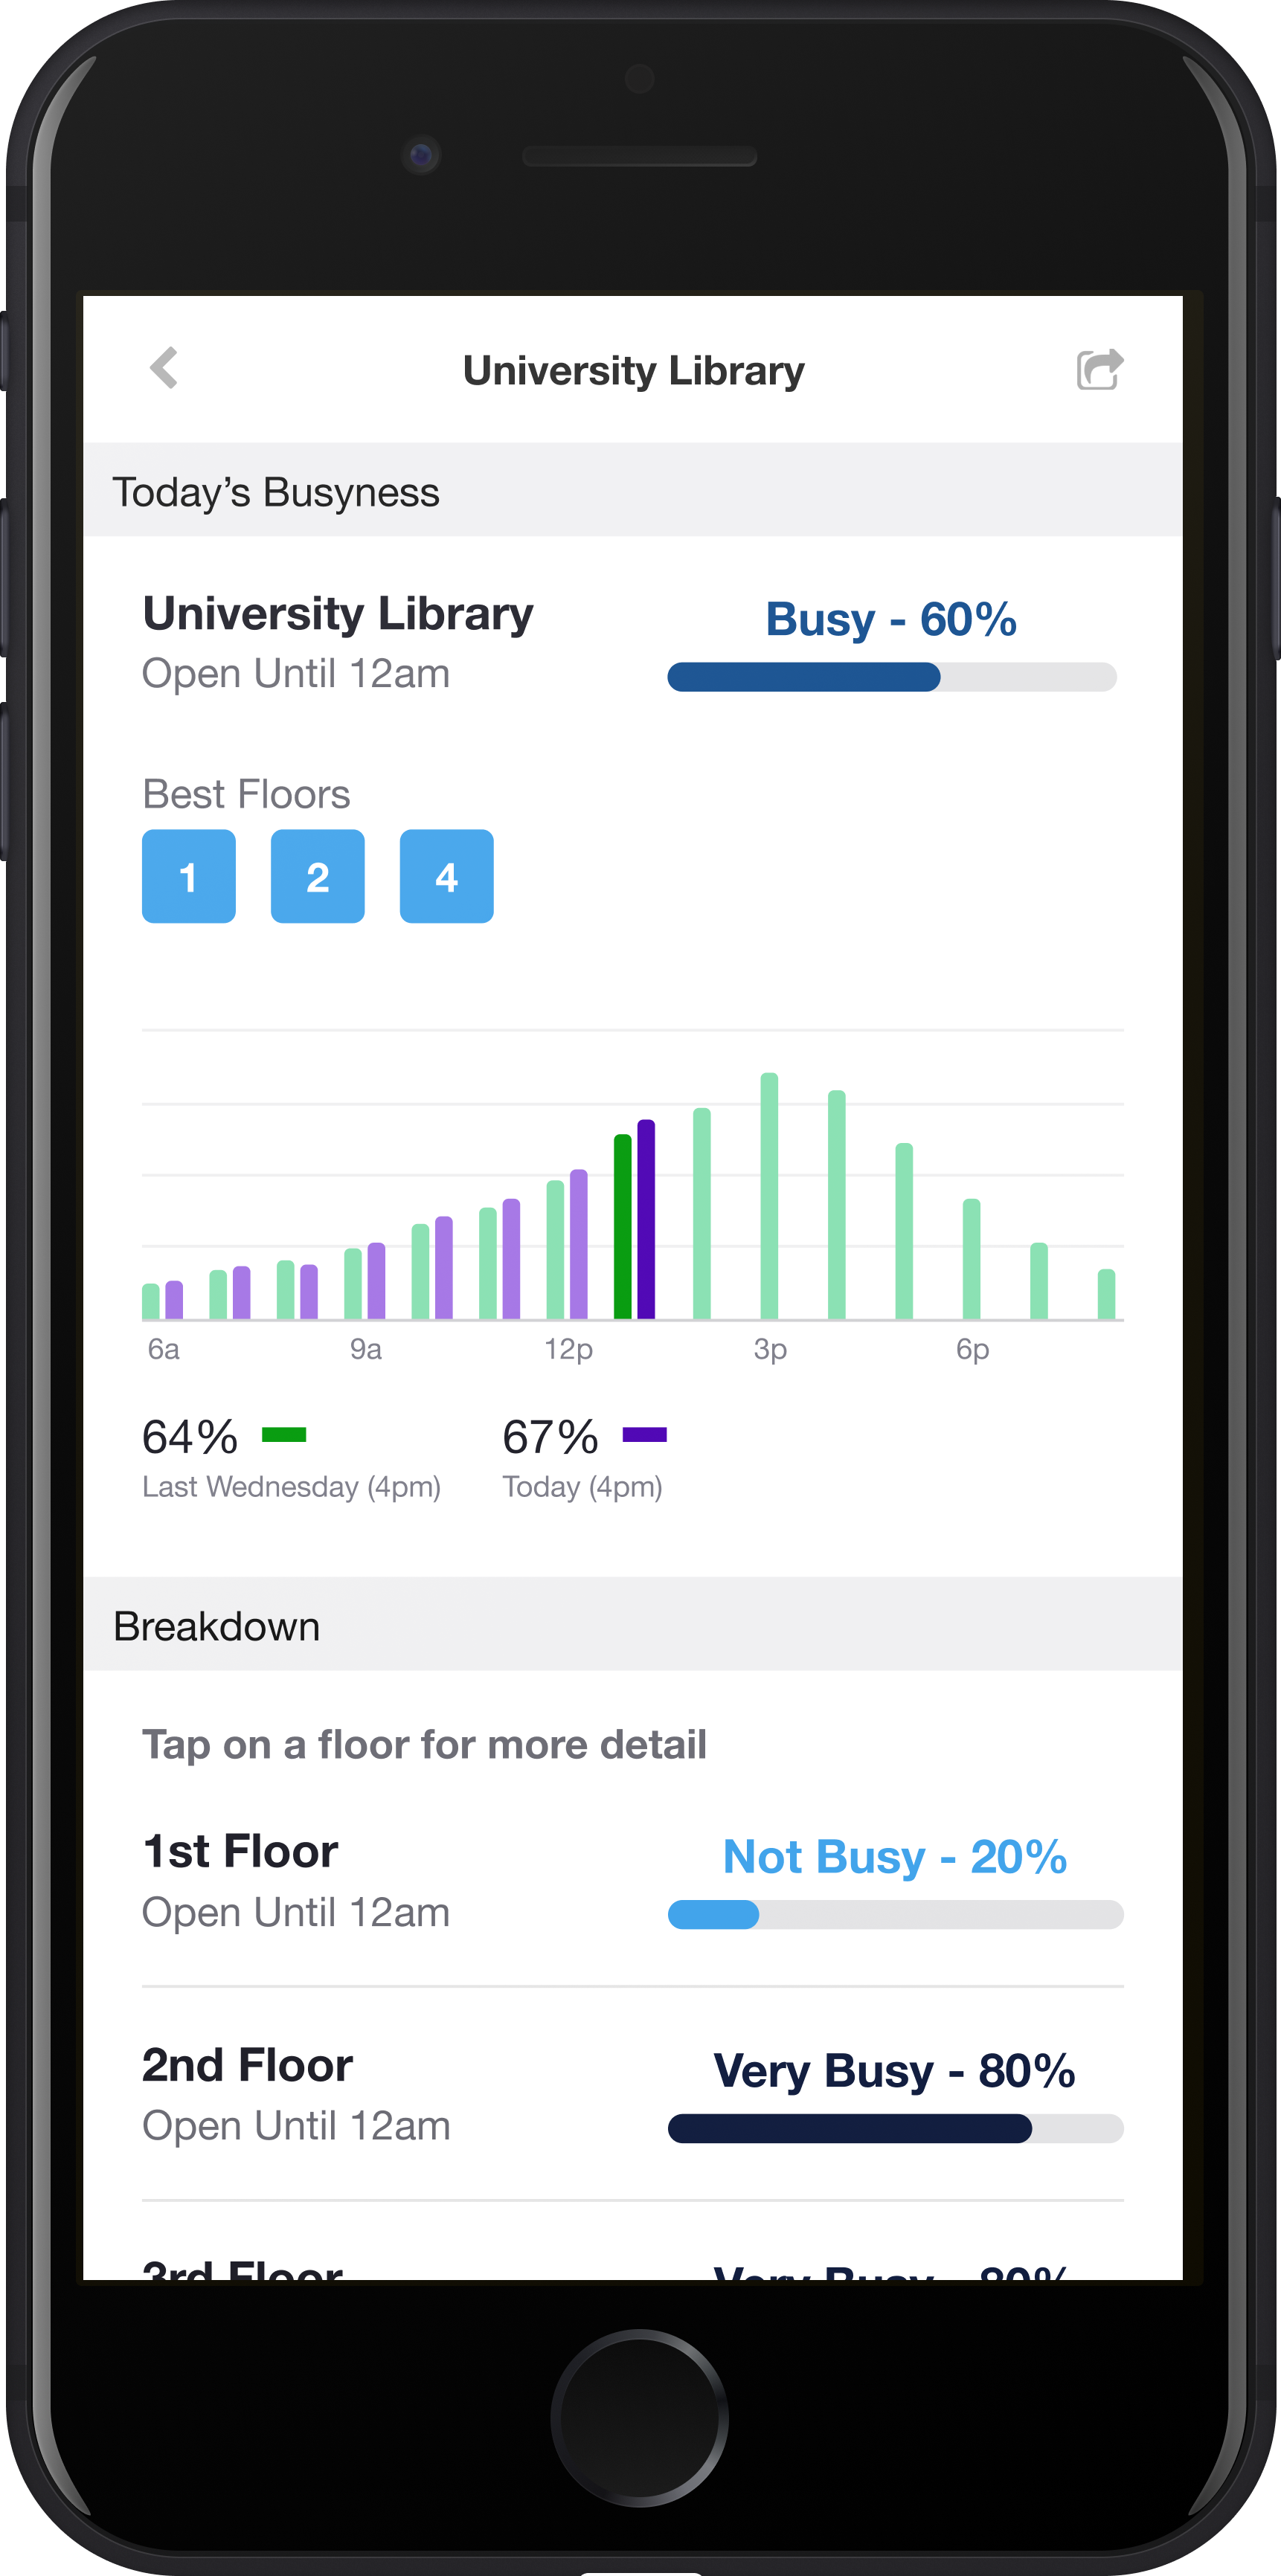
\includegraphics[width=0.4\columnwidth]{./images/waitz.png}
%     \captionof{figure}{Waitz UI}
%     \label{fig:waitz_ui}
%     \medskip
% \endgroup
% \medskip

\noindent However, their application is relatively simple as they did not use this data to forecast the "busyness" of locations or make predictions. Instead, it seems that they focused more on data collection and visualization. As a result, we thought it would be interesting to implement a similar tool for our campus; in the process, we hoped discover if there are any timeseries patterns we can exploit to provide useful information for students.

\subsection{Literature}

\noindent Unsurprisingly, there have been several attempts at using machine learning to determine "crowdedness" or "busyness". One of the benefits of searching through published work was being able to pick up on vocabulary within the field of research, making it easier to find other works. \\

\noindent We found that published work refers to this topic as "occupancy prediction" using "Wifi probing"\cite{wang2018occupancy}. Specifically, the work published by Wang et. al. determined five main characteristics in their occupancy prediction project. They realized their collected data had a "time-series characteristics" \cite{wang2018occupancy}, validating our hypothesis that occupancy is relative to time of day, as well as the idea that past data can feasibly predict future data. While this may be trivial to the overall project, it was a source of confidence for our project as it implied we could successfully build a reasonably performing model. \\

\noindent The researchers implemented a "Markov-based feedback Recurrent Neural
Networks (M-FRNN)" \cite{wang2018occupancy} model as part of their project to predict occupancy. They described the most basic neural network as having 3 layers, with the input layer accepting a vector of hashed MAC addresses, at a given time t. Moreover, they acknowledged that their raw data had fluctuations and noise that could potentially "deteriorate the prediction accuracy" \cite{wang2018occupancy}. To avoid this, they added a feature layer between the input and hidden layer, which calculates the "transfer probabilities" for every given MAC address at time t\cite{wang2018occupancy}. They describes their matrix of transfer probabilities (TPMI) as: 

\begin{gather}
 TPMI
 =
  \begin{bmatrix}
   X_{k}^{i-o} & X_{k}^{i-i}\\
   X_{k}^{o-o} & X_{k}^{o-i}\\
   \end{bmatrix}
\end{gather}

\noindent where each element is a conditional probability. For example, $X_{k}^{i-o}$ refers to the conditional probability 

\begin{equation}
    \begin{split}
        X_{k}^{i-o} = \frac{\sum{\text{from in to out}}}{\sum{\text{from in to in}} + \sum{\text{from in to out}}}
    \end{split}
    \label{eq:}
\end{equation}

\medskip
\noindent They then use the quantities $X_{k}^{o-i}$ and $X_{k}^{i-i}$ as an updated input for their hidden layer. The output of the hidden layer is sent to something called the Context layer (serving as a short-term memory), which then feeds back into the hidden layer at each run of the network \cite{wang2018occupancy}. Their error function was simply a square of the actual occupancy subtracted from the predicted occupancy\cite{wang2018occupancy}. \\

\noindent Another extremely important takeaway from this paper was the model assessment. Previously, we were only familiar with mean absolute percentage error (MAPE) and mean absolute error (MAE) as metrics. However, the researchers pointed out that these metrics "assume that an accurate prediction should have exactly
same number as the observed occupants number" \cite{wang2018occupancy}. This is usually harmful to model assessment because a small tolerance should be granted. As long as the difference is minute, an "incorrect" output value can still be classified as an accurate prediction. Hence, they used a metric called the X-accuracy. They found that their M-FRNN model performed very well when the tolerenace (X) was set to 3, providing 80\% accuracy on just the 3rd day. \\

\noindent Studying this paper was very crucial for us, as it gave us a starting point and some needed insight in how to approach the model formation. It was also encouraging to see that an example of a how typical machine learning model (ANN in this case) could be modified to account for the potential problems found in the data or problems inherent to the project itself. 



\section{Methodology}
\noindent The methodology for realizing this project has 4 main steps: data collection, data processing, data analysis, and user interface. All of these steps are feasible by using the correct hardware with correct machine learning tools.

\subsection{Feasibility}
\subsubsection{Data Collection} Data collection is the lowest level in the process and it is achieved by using ARM based Raspberry Pi Zero computers since they have builtin bluetooth and WIFI chips. Besides having the WIFI chip as an hardware, the WIFI chip itself should be supporting the "monitoring" mode for monitoring the wireless traffic. The WIFI chip of Raspberry Pi Zero also has this monitoring feature that enables the data collection for the project.

\begingroup
    \center
    \medskip
    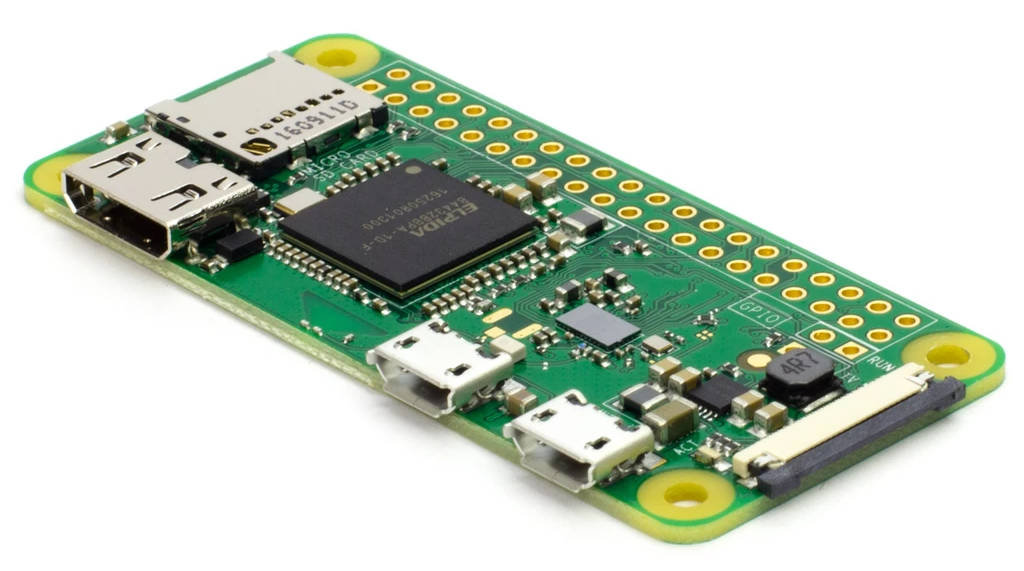
\includegraphics[width=0.6\columnwidth]{report/interim_report/images/raspi.png}
    \captionof{figure}{Raspberry Pi Zero used for data collection}
    \label{fig:raspi}
    \medskip
\endgroup

\noindent The  Raspberry Pi Zero computer is running a special version of the Linux operating system and this also helps us with the data collection since Linux natively supports the \texttt{dumpcap} tool, which was used to collect the data packages in the air. Further details related to the \texttt{dumpcap} network traffic dump tool can be found  \href{https://linux.die.net/man/1/dumpcap}{here}.\\

\noindent When a WIFI chip is in the monitoring mode it is not capable of collecting private data since WIFI traffic between devices and the routers are already encrypted with some sort of password protection. That being said, we can still get various data regarding the source and destination of the data packages. These non-private information is enough for our project since we want to be able to approximately count the number devices and people in a space rather than spying on personal data. The following are the data fields that can be collected while monitoring WIFI signals in the monitoring mode:

\begin{itemize}
    \item \texttt{frame.number}
    \item \texttt{frame.time}
    \item \texttt{wlan.addr}
    \item \texttt{wlan.ta}
    \item \texttt{wlan.ra}
    \item \texttt{wlan.sa}
    \item \texttt{wlan.da}
    \item \texttt{wlan.bssid}
    \item \texttt{wlan.fc.type}
    \item \texttt{wlan.fc.type\_subtype}
    \item \texttt{radiotap.channel.freq}
    \item \texttt{radiotap.datarate}
    \item \texttt{radiotap.dbm\_antsignal}
\end{itemize}
\medskip
\noindent Here, \texttt{frame.number} and \texttt{frame.time} are the fields that contain date time information about the data package. These fields are useful for creating a time series data set out of the collected network traffic. The fields that start with \texttt{wlan} have the information regarding the source and destination of the data packets. This is information is given in the form of Media Access Control (MAC) addresses per each packet. This information is useful for counting and classifying the number of devices nearby to measure the crowdedness because MAC addreses are unique to every device and there are no two different WIFI devices with the same MAC address. Finally, the fields that start with \texttt{radiotap} have information regarding the signal strength, wireless frequency, and the data rate that channel support. Again, these fields are useful for understanding the proximity of the WIFI device and making decisions about whether to include or not to include certain devices into calculations.\\

\noindent For demonstrating the functionality of the system, more than 1 million data packages were collected over a week. The preview of the pandas dataframe that holds the data shows the collected data in Figure \ref{fig:pandas}.

\begingroup
    \center
    \medskip
    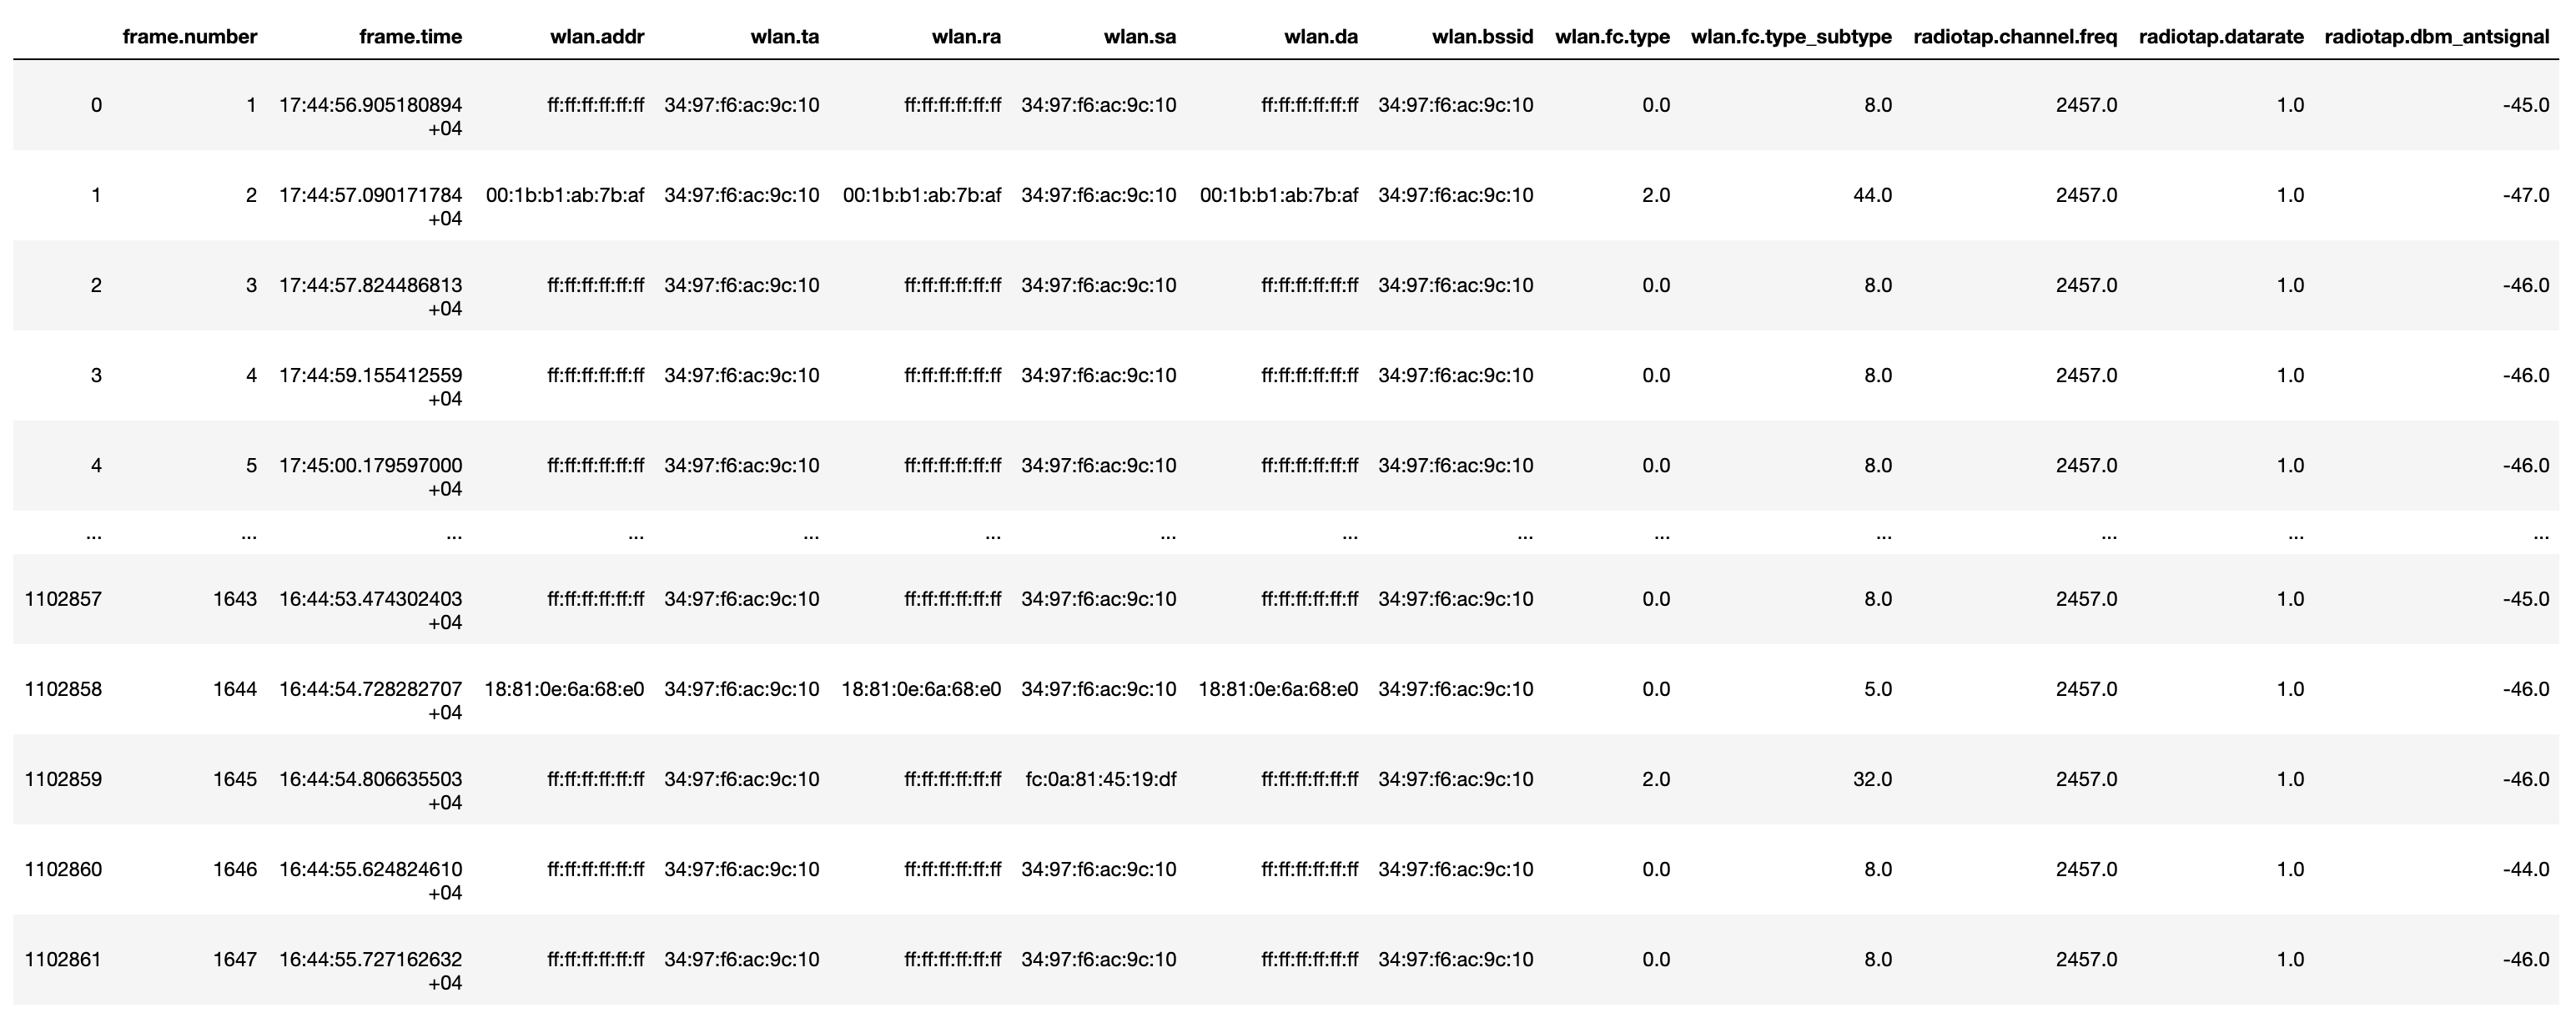
\includegraphics[width=\columnwidth]{report/interim_report/images/pandas.png}
    \captionof{figure}{Preview of the pandas dataframe created with the collected network traffic}
    \label{fig:pandas}
    \medskip
\endgroup


\subsubsection{Data Processing} 
After the data collection, the data can be processed to remove invalid and empty values as usual. Later, the MAC addresses collected under the \texttt{wlan} fields should be validated using the MAC address rules defined by the Institute of Electrical and Electronics Engineers (IEEE). Later, the MAC addresses should be converted into their decimal representations. Normally, MAC addresses are hexadecimal values and they are stored as strings since they contain letters inside them. However, we cannot use strings with machine learning algorithms and we need to get the decimal representation of each mac address to use the machine learning algorithms for analysing data in the next step. Thus, the data processing step is crucial for having high quality data for training. \\

\subsubsection{Data Analysis} 
% include information about some nuances we need to think about or we can extract. For example, do we have to worry about someone "passing by" if their MAC address was available for just a small bit of time. 


\begingroup
    \center
    \medskip
    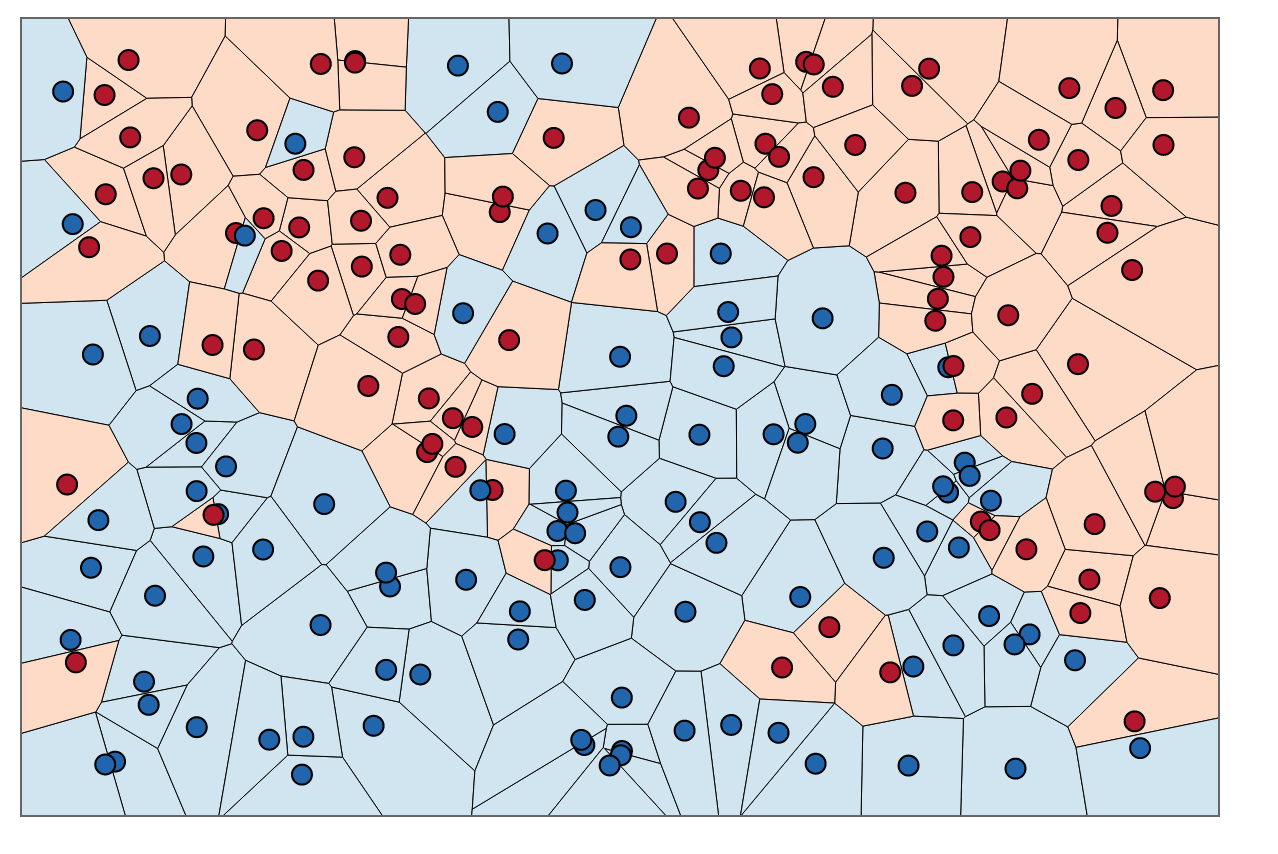
\includegraphics[width=\columnwidth]{report/interim_report/images/clustering.png}
    \captionof{figure}{Illustration for clustering the WIFI devices nearby}
    \label{fig:clustering}
    \medskip
\endgroup



\subsubsection{User Interface} 
After the data collection, processing, and analysis steps are completed, the final step is having a very basic user interface for presenting the predicted data. For achieving this, we are going to use \href{https://getbootstrap.com/}{Bootstrap library} for designing the user interface itself and use the PHP language for making the webpage dynamic that it can update the data shown with the real time data. A SQLite database will be used to store the collected and processed data. We already have a web hosting and a web domain (\href{https://nyuad.app/}{nyuad.app}) that we already have for other projects as well. So, the app is going to be located at \href{https://nyuad.app/flyway/}{nyuad.app/flyway}.

\begingroup
    \center
    \medskip
    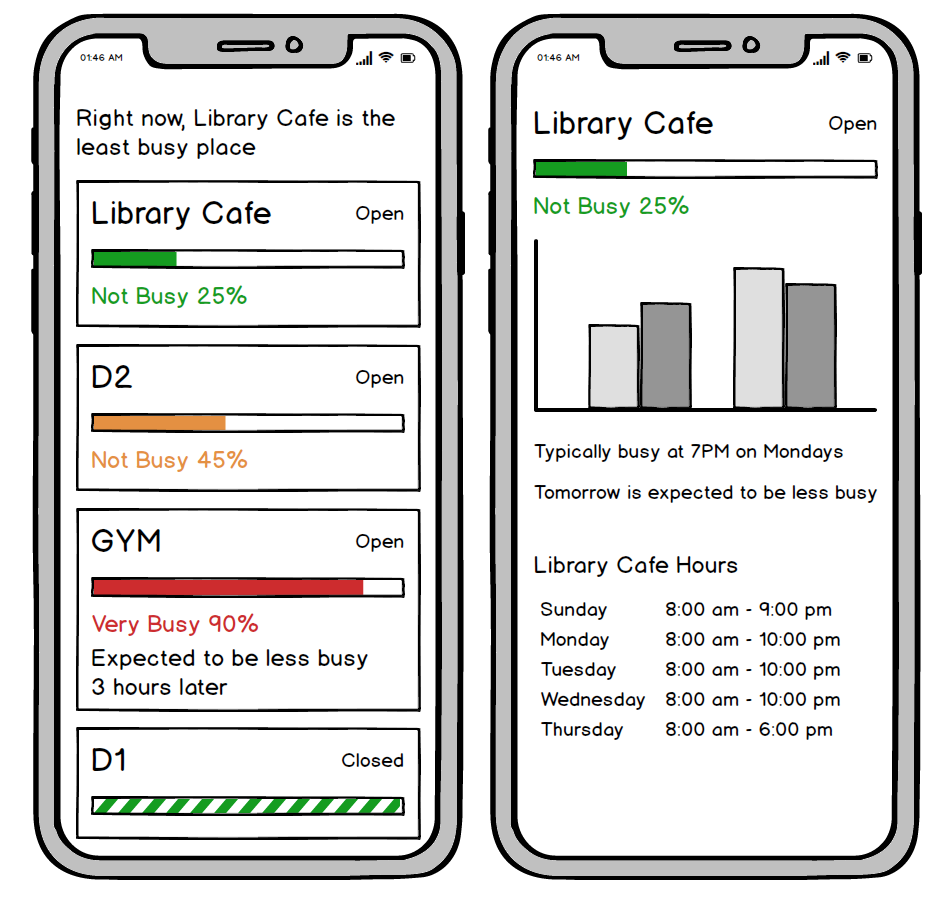
\includegraphics[width=0.6\columnwidth]{report/interim_report/images/ux.png}
    \captionof{figure}{Proposed user interface}
    \label{fig:ux}
    \medskip
\endgroup

\subsubsection{Feasibility Conclusion} 
We already figured out the exact tools and software that we need to use to make this project possible. We also have some previous experience with these software and tools from previous projects. Therefore, we believe that this project is feasible to build by using the tools and knowledge available to us.




\subsection{Applicability to Solving the Problem}


%%%%%%%%%%%%%%%%%%%%%%%%%
%% Experimental Method %%
%%%%%%%%%%%%%%%%%%%%%%%%%

%%%%%%%%%%%%%
%% Results %%
%%%%%%%%%%%%%

%%%%%%%%%%%%%%%%
%% Discussion %%
%%%%%%%%%%%%%%%%

\printbibliography

\end{document}

%%%%%%%%%%%%%%%
%% Equations %%
%%%%%%%%%%%%%%%

% \begin{equation}
%     \begin{split}
%         X &\texttt{\char`\~} Poisson(\lambda) \\
%         \\
%         P(X=k) &= \frac{\lambda^k e^{-\lambda}}{k!} \\
%         \\
%         \EX(k) &= e^{-\lambda}\sum_{k=1}^{\infty} \frac{\lambda^n}{(n-1)!}\\
%         \\
%         &= e^{-\lambda}\lambda\sum_{k=1}^{\infty} \frac{\lambda^{k-1}}{(k-1)!}\\
%         \\
%         &= e^{-\lambda}\lambda\sum_{n=0}^{\infty} \frac{\lambda^{n}}{(n)!}\\
%         \\
%         &= e^{-\lambda}\lambda e^{\lambda} = \lambda\\
%     \end{split}
%     \label{eq:mutual}
% \end{equation}


% \begin{equation}
%     \begin{split}
%         \lambda = \frac{\sum_{i=1}^{n}D_i}{n}
%     \end{split}
%     \label{eq:poisson_distribution}
% \end{equation}

%%%%%%%%%%%
%% Table %%
%%%%%%%%%%%

% \begingroup
%     \medskip
%     \centering
%     \def\arraystretch{1.5}
%         \begin{tabular}{lcc}
%             \toprule
%             & Random Network & Scale-Free Network \\
%             \midrule
%             Avg. of Avg. Degree    & 3.9988    &  4.0035   \\
%             Var. of Avg. Degree    & 7.6800$\times 10^{-7}$ & 3.1156$\times 10^{-6}$  \\
%             Avg. of Avg. Distance  & 5.5694 & 5.0935    \\
%             Var. of Avg. Distance  & 1.5507 & 0.5377   \\
%             \bottomrule
%         \end{tabular}
%     \captionof{table}{Statistics of fifty runs where \\ n = 5,000, e = 10,000}
%     \label{table:fifty_runs}
%     \medskip
% \endgroup
